\documentclass[12pt, english,a4paper]{article}

\usepackage[T1]{fontenc}
\usepackage[latin9]{inputenc}
\usepackage[english]{babel}
\usepackage{lmodern}
\usepackage{hyperref}
\usepackage{color}
\usepackage{url}
\usepackage{verbatim} 

\usepackage{graphicx}
\usepackage{float}
\usepackage{amsmath}


\graphicspath{{./figures/}}
\begin{document}


\title{Click-stream Data Analysis of Web Traffic}
\author{Riivo Kikas, Karl Potisepp}
\date{\today}
\maketitle


\begin{abstract}
In this paper, we conduct a case study of mining frequent user access patterns from web log files. Our primary objective was to discover the most frequent browsing patterns by analyzing the visitors' browsing sessions. The nature of pattern mining carried out was mainly exploratory, concentrating on frequent item sets and sequence mining. To achieve this, we eliminated irrelevant data from the access logs, extracted user sessions and searched them interesting usage patterns. During this work we experimented with several frequent itemset mining algorithms and tools. As a result of our work we provide this case study and some statistics about the usage patterns of the public web site of the Faculty of Mathematics and Computer Science of the University of Tartu.
\end{abstract}


\tableofcontents


\section{Introduction} 
Understanding how users navigate and browse through web sites is important in many aspects, such as content recommendation,
personalization and targeted advertising. Even more, it helps to understand users' needs and provides real world input to better organization of content and structure. Web server log files can provide important insight to the users' behavior, because from this data one can reconstruct a reasonably accurate overview of how users navigate their way to whatever content they desire. Coupled with data mining algorithms it is therefore quite probable that important knowledge can be gained.

As an experimental case study, we studied the web access logs from the public web site of the Faculty of Mathematics and Computer Science of the University of Tartu\footnote{\url{http://math.ut.ee}}. Our aim was to try and find meaningful use-cases from log files and identify possible bottlenecks in the presentation layer and provide some input for user interface redesign.





\section{Data preparation} 
For each time an user visits a web page, a piece of information is typically stored in a web server's log file. When user navigates around a website, all such pieces of information (alternatively called requests or clicks) form a session (click-stream). We consider user's single purposed visit  (i.e. a search for a phone number or information about entrance exams) as a session and associate each user click with a particular session. 

Input data is stored in website log files, namely in Common Log Format\cite{ref_clf} format. Each log entry consists of:  (i) User's IP address, (ii) Access time, (iii) Request method (\emph{GET}, \emph{POST}), etc), (iv) URL of the page accessed, (v) Protocol (typically HTTP/1.0), (vi) Return code, (vii) Number of bytes transmitted\ref{log_sample}.

Log files contain all HTTP requests made to the web server, including requests for downloading images and style sheet documents attached to the web pages served.

\begin{figure}[h]
{\tiny
\begin{verbatim}
192.168.1.245 - - [13/Sep/2009:04:07:56 +0300] "GET /ati/struktuur/tiiger HTTP/1.0" 200 19828
192.168.1.215 - - [13/Sep/2009:04:09:30 +0300] "GET / HTTP/1.0" 200 13511
192.168.1.215 - - [13/Sep/2009:04:12:02 +0300] "GET /103369 HTTP/1.0" 200 17367
192.168.1.215 - - [13/Sep/2009:04:14:40 +0300] "GET /varia/itinfo HTTP/1.0" 200 19411
\end{verbatim}
}
\label{log_sample}
\caption{Example of a log file}
\end{figure}

Two important tasks must be performed before click-stream data from \emph{CLF} files can be used for analyzing: data cleaning and session identification.







\subsection{Data cleaning}
Since log files contain all requests made to the server, we need to extract only relevant requests and eliminate others. When filtering requests from log files, following rules were applied:

\begin{itemize}
\item Only requests to the public site are considered. Requests to personal home pages (URLs starting with ~) are discarded. Also, all static content files that were used by web pages were removed, such as image files, JavaScript and CSS documents. \\ The server also had had special error page URL, that the user was redirected to when they tried to access a non-existent resource. We eliminated this kind of access requests, as these are not initially made by users. It must be noted that the request for the original page that caused the server to redirect the user remains in the log file.
  
\item All other HTTP request types besides POST and GET were ignored. We noticed that there were regular OPTIONS requests, that most probably were made by some automated monitoring tool. 
  
\item We composed a blacklist of of IP addresses, whose requests were all ignored. An IP-address was added to blacklist, if there was a request made from the IP address to access \emph{robots.txt} file. Namely, we believe that only automated indexers request robot.txt and therefore we can ignore all subsequent requests from those IP-s, since we are only interested in how a human user perceives the web site. 
\end{itemize}


Moreover, we modified requested URLs by removing query string attributes (the part of the URL that starts with \emph{?}). We assumed that typically URLs identify a distinct page and query-string some operation or action on it. This helped us to reduce the number of different URLs while preserving meaningful information about the usage patterns.

After performing all the procedures described above, the log files contained only information about the HTTP requests originating from intentional clicks made by the users on pages. These clicks can be grouped into users' click-streams.











\subsection{Session identification}
The next step was to group user requests made during one visit into sessions. A user session is defined as a sequence of temporally compact accesses by a user \cite{on_mining_logs}.

Generally, this can be done by providing a cookie to each user with some generated unique identification number and then logging each request and the cookie ID simultaneously. However since CLF does not store an explicit session ID, and since we could not modify the existing software stack, we had to reconstruct user sessions from log files.  

As a solution, we used a timeout based method to group requests into sessions. We consider a sequence of requests from the same IP address ordered by time to be in same session, if the time between consecutive requests (clicks) is no more than $t = 30$ minutes. If time between requests exceeds $30$ minutes, we consider these requests to be part of a new session. While this method is probably not the best, we consider it sufficient as it mimics the way session timeouts are measured on many web sites. We also consider it reasonable to assume that if an user has not interacted with the server for more than $t$
minutes, any new interaction from an user from the same IP address can be thought of as a new use case scenario.







\subsection{Statistics about the logs} 
The log files contained info about requests made to the server from August to December 2009, with October data missing. In total, log files contained $544237$ requests, of which $122822$ remained after eliminating uninformative lines. These requests were grouped to $35952$ sessions. The average session length was $3.4$ clicks. Distribution of user session length can be seen on figure \ref{session_len}. Requests involved $2059$ distinct URLs.

\begin{figure}[H]
  \centering
      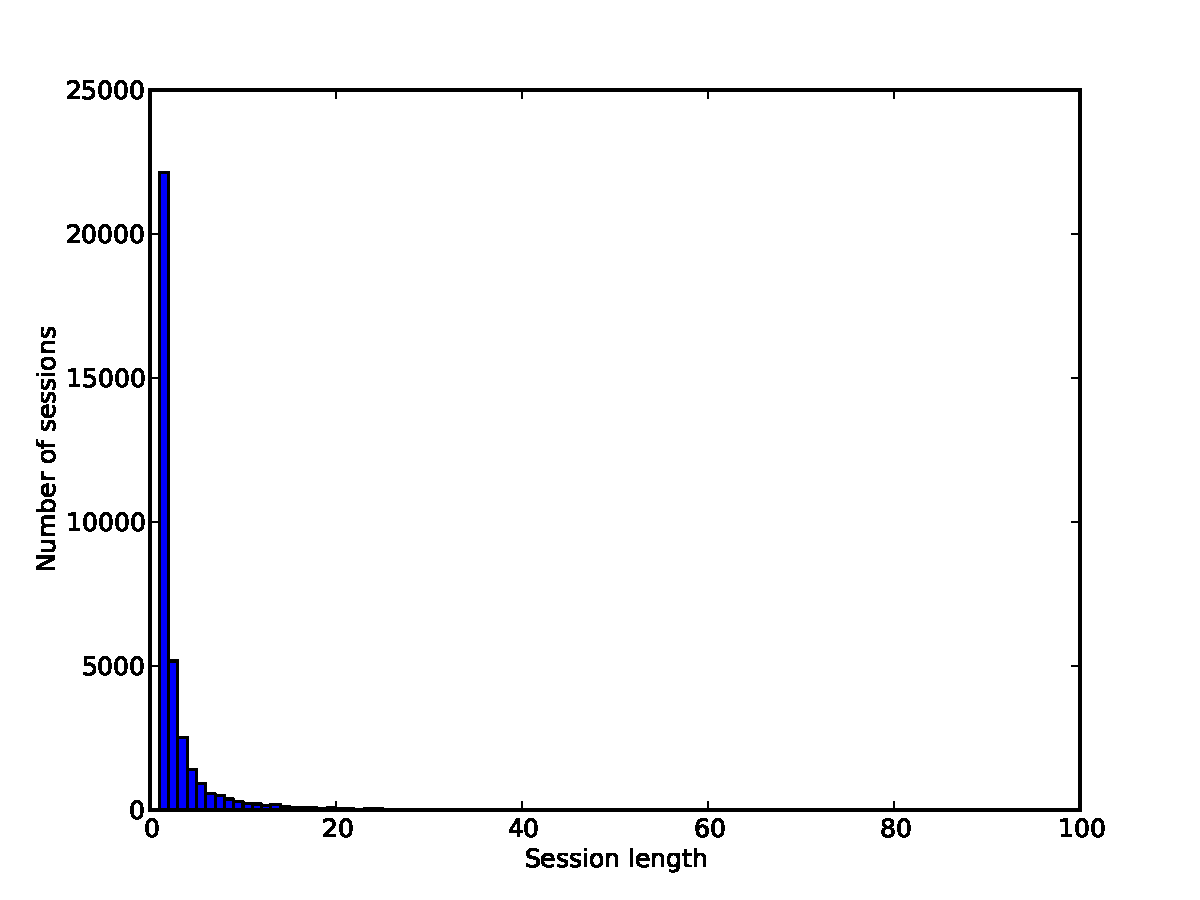
\includegraphics[width=0.9\textwidth]{session_len}
  \caption{Session length histogram}
  \label{session_len}
\end{figure}









\section{Frequent item sets} 
From the perspective of web site design and browsing sessions, the most important question is whether or not there are groups of pages users tend to visit together. The presence of such kinds of groups can give a web designer valuable insight into how people use the web site. For example, content split on separate pages but still often viewed together can be merged to achieve a smoother browsing experience.

We approached the task of identifying such groups by thinking of every page as a unique \emph{item}, which then form sets, each containing pages visited during one browsing session. To find pages that are frequently visited together, we searched among these sets for subsets of pages that frequently appear together. The problem now was deciding when a subset of pages is frequent. We solved this by using a set mining \cite{frequent_item_set_mining} concept called \emph{support}.

Support is a number that shows how frequently a subset appears in all item sets. Using this concept, it is trivial to eliminate subsets that are not common (and therefore not interesting). The only problem is that there is no magic bullet solution to choosing the 'right' support threshold. A value too high does not provide insight into more specific subsets, a value too low results in too much non-frequent garbage.
\begin{figure}[H]
  \centering
      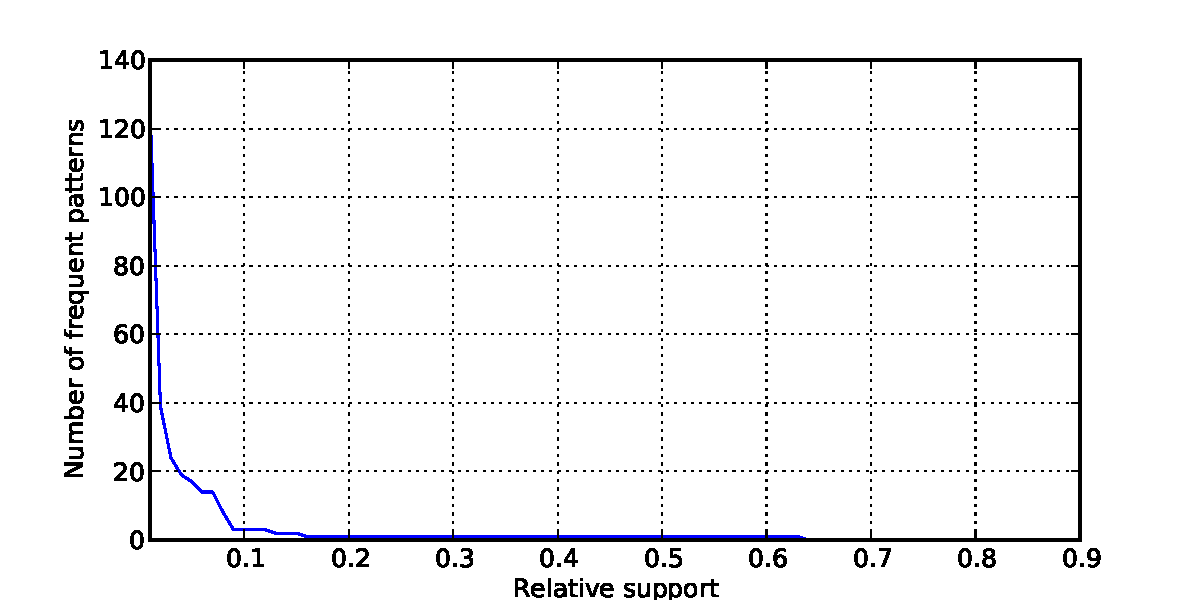
\includegraphics[width=0.9\textwidth]{apriori_closed_itemset_count}
  \caption{How rule support changes number of frequent closed itemsets}
\end{figure}


However even if we manage to choose an optimal value for the support threshold, after filtering out all the infrequent subsets, some redundancy remains in the results. It is easy to see that if a set of 5 pages appears frequently throughout the sessions, all 4 page subsets of that set appear at least as frequently. To eliminate this kind of noise, we used the Apriori algorithm \cite{apriori} to first find all frequent item sets, from which we then extracted \emph{closed itemsets}.

In addition to the difficulties in choosing an ideal support threshold, there are other problems with this approach to detecting pages frequently requested during one session. While we can easily find groups of pages that are probably viewed together, much more insight could be gained if we knew the order in which the pages were navigated. Knowing this we would also gain information on how the users find what they need on the site. Similarly, if an user visits a page several times during one session, this fact is not known to us. Using \emph{sequential item sets} solves these problems.

From \ref{frequent_patterns} , it can be seen that homepage(\emph{avaleht}) is on of the most frequently accessed resource, which is obvious. The advantage of frequent pattern mining can be explained with the itemset where pages \emph{avaleht, 15208, inimesedInstituudid} are present together: it shows that navigation is mostly done starting from homepage and also that official peoples listing page (\emph{inimesedInstituudid}) is used as a hop to go to computer science faculty members listing page(\emph{1508}).  The order of pages travelled is not obvious, but we now here that the navigation other way around is not possible, as the links do only exist one-way. This problem can be used by mining frequent sequential patterns.

\begin{figure}[H]
  \centering
\begin{tabular}{ r | l }
Support & frequent itemset \\ \hline
0.63 & avaleht \\ \hline
0.13 & 15213 \\ \hline
0.1 & inimesedtudengid \\ \hline
0.1 & avaleht, 15213 \\ \hline
0.09 & inimesedInstituudid \\ \hline
0.09 & 15208 \\ \hline
0.09 & avaleht, inimesedtudengid \\ \hline
0.09 & 15205 \\ \hline
0.08 & avaleht, inimesedInstituudid \\ \hline
0.08 & 15213, inimesedtudengid \\ \hline
0.08 & avaleht, 15213, inimesedtudengid \\ \hline
0.08 & avaleht, 15208 \\ \hline
0.07 & 15208, inimesedInstituudid \\ \hline
0.07 & avaleht, 15208, inimesedInstituudid \\ \hline
\end{tabular}
  \caption{Frequent closed itemsets having more than relative support=$0.06$. Support value is given with rounding error and closed itemsets were found using absolute support.}
  \label{frequent_patterns}
\end{figure}

Analyzing these results gives little new information. As expected, the most frequent pattern is \emph{avaleht}, which is the root page of the faculty's web site. The second most frequent, with relative support almost six times less, is the page containing the names of all students currently pursuing degrees in majors that are tied to the Computer Science and Mathematics faculty - \emph{15213}. In the log files this URL was sometimes followed by a list of HTTP GET attributes used to specify what information should be shown on the page. However since during the extraction step we removed these attributes from all URLs, we could not analyze the exact usage of this page further - such knowledge can probably be obtained from the log files of the database providing the students' data.


\section{Frequent sequential patterns}
Simply by listing all frequent item sets we will not see much of how users actually use the website. This is because of two reasons. First, frequent item sets do not capture the order of pages visited. Secondly, information about multiple page visits is lost constructing item sets.

This problem can be solved by mining frequent sequential item sets. Sequential pattern mining is about mining frequent event sequences from databases, which means that we are searching for sequences of clicks that more often than not are followed by each other. Frequent sequences can be used to see how users actually tend to navigate and reach some desired resource.

\begin{figure}[H]
  \centering
      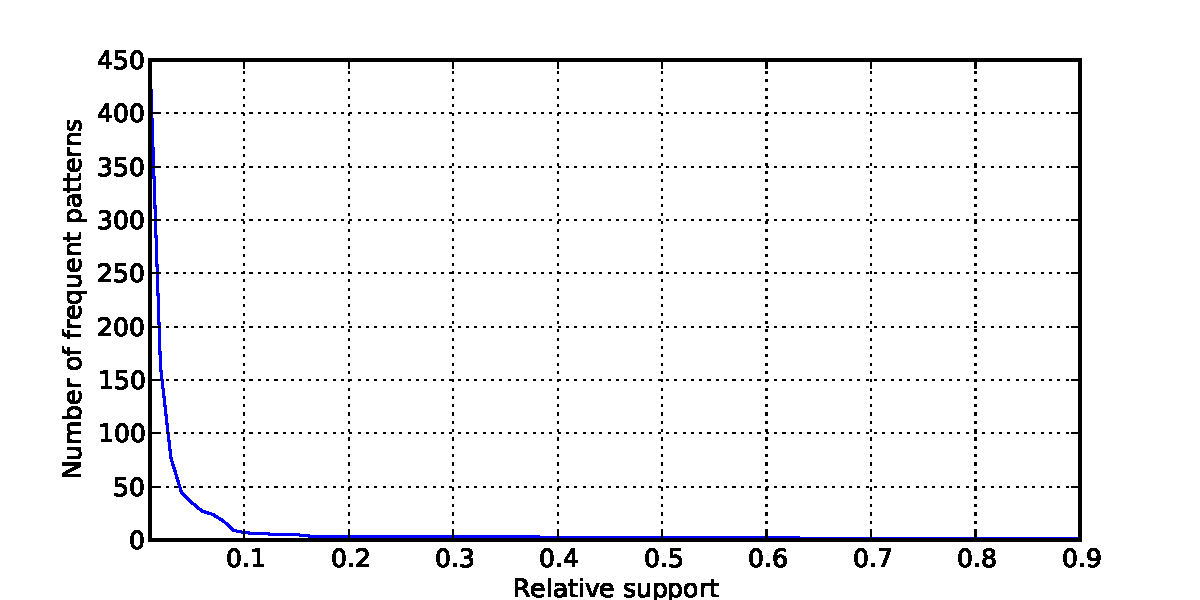
\includegraphics[width=0.9\textwidth]{sequential_itemset_count}
  \caption{Number of frequent sequential patterns depending on relative support}
\end{figure}


To mine frequent patterns from our dataset, we used an \emph{a priori}-based frequent item sequence miner that uses a trie to store the candidates\cite{seq_apriori}.


Compared to simple frequent frequent itemsets, sequential patterns yield to more existing results (\ref{frequent_patterns}). First thing to notice is the continuous main-page refreshing with quite big time intervals. Our guess is that it caused by the people in faculty who have set faculty website as their home page in browser and when they open up new browser window, home page is opened. There is no better explanation for this phenomenon as the main page is currently pretty static had seldom updated.

Most important result from usability point of view  are the patterns where users visit page \emph{inimesedInstituudid}. Users spend relatively little time on this page, for example in sequence
\[ 
\overset{6.0}{avaleht} \rightarrow \overset{3.0}{inimesedInstituudid} \rightarrow \overset{30.0}{15208} 
\]
it is only  3 seconds for as all users' median time, but the page user landed after visited takes 30seconds. The reasons for is that page  \emph{inimesedInstituudid}  is only a navigational page - it holds links to other pages. This page can be eliminated, for example including the links on the main page somehow, possibly with a drop-down menu or adding directly.



\begin{figure}[H]
  \centering
\begin{tabular}{ r | l }
Support & frequent sequential pattern \\ \hline
0.63 & $ \overset{17.0}{avaleht} $ \\ \hline
0.38 & $ \overset{513.0}{avaleht} \rightarrow \overset{137.0}{avaleht} $ \\ \hline
0.16 & $ \overset{592.5}{avaleht} \rightarrow \overset{600.5}{avaleht} \rightarrow \overset{237.5}{avaleht} $ \\ \hline
0.16 & $ \overset{28.0}{ati} $ \\ \hline
0.13 & $ \overset{11.0}{15213} $ \\ \hline
0.1 & $ \overset{9.5}{15213} \rightarrow \overset{23.0}{15213} $ \\ \hline
0.1 & $ \overset{4.0}{inimesedtudengid} $ \\ \hline
0.09 & $ \overset{4.0}{inimesedInstituudid} $ \\ \hline
0.09 & $ \overset{42.0}{15208} $ \\ \hline
0.09 & $ \overset{110.5}{avaleht} \rightarrow \overset{117.0}{15213} $ \\ \hline
0.09 & $ \overset{8.0}{avaleht} \rightarrow \overset{4.0}{inimesedtudengid} $ \\ \hline
0.09 & $ \overset{255.0}{ati} \rightarrow \overset{179.5}{ati} $ \\ \hline
0.09 & $ \overset{21.0}{15205} $ \\ \hline
0.08 & $ \overset{4.0}{inimesedtudengid} \rightarrow \overset{8.0}{15213} $ \\ \hline
0.08 & $ \overset{7.0}{avaleht} \rightarrow \overset{4.0}{inimesedInstituudid} $ \\ \hline
0.08 & $ \overset{429.0}{avaleht} \rightarrow \overset{474.0}{avaleht} \rightarrow \overset{401.0}{avaleht} \rightarrow \overset{171.5}{avaleht} $ \\ \hline
0.08 & $ \overset{7.0}{avaleht} \rightarrow \overset{4.0}{inimesedtudengid} \rightarrow \overset{7.5}{15213} $ \\ \hline
0.08 & $ \overset{81.0}{avaleht} \rightarrow \overset{67.0}{15213} \rightarrow \overset{69.0}{15213} $ \\ \hline
0.07 & $ \overset{97.5}{avaleht} \rightarrow \overset{73.0}{15208} $ \\ \hline
0.07 & $ \overset{4.0}{inimesedtudengid} \rightarrow \overset{7.0}{15213} \rightarrow \overset{18.0}{15213} $ \\ \hline
0.07 & $ \overset{4.0}{inimesedInstituudid} \rightarrow \overset{31.5}{15208} $ \\ \hline
0.07 & $ \overset{8.0}{avaleht} \rightarrow \overset{4.0}{inimesedtudengid} \rightarrow \overset{7.0}{15213} \rightarrow \overset{18.0}{15213} $ \\ \hline
0.07 & $ \overset{8.0}{avaleht} \rightarrow \overset{19.0}{15205} $ \\ \hline
0.07 & $ \overset{6.0}{avaleht} \rightarrow \overset{3.0}{inimesedInstituudid} \rightarrow \overset{30.0}{15208} $ \\ \hline
0.07 & $ \overset{9.0}{15213} \rightarrow \overset{20.0}{15213} \rightarrow \overset{7.0}{15213} $ \\ \hline
0.06 & $ \overset{59.5}{oppetootunniplaanid} $ \\ \hline
\end{tabular}
  \caption{Frequent sequential patterns with time decorations. Time is given in seconds and is calculated by taking median value of time spent on that page that contains specified rule. }
  \label{frequent_patterns}
\end{figure}



\subsection{Page access times}
Because the log files contain time and date info for every request made by the user, we know the time of each mouse click the user made (to a precision of 1-2 seconds, taking into account the time it takes for a request to reach the server). Knowing this we can find how much time users actually spend on a web page by calculating the time interval between two clicks. For every page, we can calculate the average time users spend on this page. However a more effective approach is to apply this method to previously found sequential patterns. Namely, for every frequent sequence found, we find all sessions that contain this sequence and calculate median time spent viewing each page in that sequence. We chose median time as we consider this more appropriate for experimental evaluation.

This method allows us to determine the pages that are visited only because of navigation and not for content. For usability reasons, such pages should be removed to reduce user clicks.





\section{Maximal reference sequences}
Path traversal pattern mining has been studied extensively to find better alternatives to regular frequent sequence mining in the context of web mining. A solution has been proposed \cite{path_patterns} that provides regular sequential patterns, but reduces the patterns only to \emph{forward reference sequences}, that is patterns that only contain forward navigations. Authors of \cite{path_patterns} say that forward references illustrate what people are looking for (e.g. destination pages) and eliminate back references from sessions.

When we applied this algorithm to our dataset, we found almost the same frequent patterns as with the regular sequential pattern mining technique. The difference was only the number of patterns found, which means that by eliminating back references and repeating pages, we find less patterns. When the number of patterns is bigger, this method helps to achieve better overview of frequent user traversal paths and target pages than the previously used method.

\section{Changes in patterns through time} 
Pattern mining can also give insight into how patterns change over time. When mining school website data, one can hypothesize how users' interest changes in time. We can presume, that since August is the pre-semester period and students might be looking for information about new professors, timetables or good seminars provided on the upcoming semester. Once the semester starts in September, it can be assumed that these kinds of aims become outdated and new behavioral patterns arise.

We split up the data set into two: August and September and compared sequential patterns found for both datasets with same relative support, s=$0.06\%$.

Results reveal that in September\ref{sep2}, a frequently accessed page was \emph{/116245}, a news item announcing semester's official introduction event and first dates for lectures. This page was not present in august data as it was published on last day of August\ref{aug2}. Contrary to this, the page listing general news(\emph{yldteated}) had support of $0.07$ in August, but in September it was below $0.06$. 

In September faculty and people listing pages(\emph{inimesedtudengid}, \emph{inimesedInstituudid}  had 3\% higher support than in August. Timetables listing page(\emph{oppetootunniplaanid})  was more frequently accessed in August than in September.

Results confirm somehow our assumptions and we conclude this method can be used to compare user interests for different periods.


\begin{figure}[H]
  \centering
\begin{tabular}{ r | l }
Support & frequent itemset \\ \hline
0.65 & avaleht \\ \hline
0.15 & 15213 \\ \hline
0.12 & inimesedtudengid \\ \hline
0.12 & avaleht, 15213 \\ \hline
0.11 & avaleht, inimesedtudengid \\ \hline
0.11 & 15213, inimesedtudengid \\ \hline
0.11 & oppetootunniplaanid \\ \hline
0.11 & avaleht, 15213, inimesedtudengid \\ \hline
0.1 & 15205 \\ \hline
0.07 & oppetoooppekavad \\ \hline
0.07 & inimesedInstituudid \\ \hline
0.07 & yldteated \\ \hline
\end{tabular}
  \caption{Frequent itemsets for August }
  \label{aug2}
\end{figure}



\begin{figure}[H]
  \centering
\begin{tabular}{ r | l }
Support & frequent itemset \\ \hline
0.67 & avaleht \\ \hline
0.14 & 15213 \\ \hline
0.12 & inimesedtudengid \\ \hline
0.12 & avaleht, inimesedtudengid \\ \hline
0.12 & avaleht, 15213 \\ \hline
0.11 & 15213, inimesedtudengid \\ \hline
0.11 & avaleht, 15213, inimesedtudengid \\ \hline
0.1 & inimesedInstituudid \\ \hline
0.09 & 15205 \\ \hline
0.09 & 15208 \\ \hline
0.09 & avaleht, inimesedInstituudid \\ \hline
0.08 & avaleht, 15208 \\ \hline
0.08 & oppetootunniplaanid \\ \hline
0.08 & 15208, inimesedInstituudid \\ \hline
0.08 & avaleht, 15208, inimesedInstituudid \\ \hline
0.07 & oppetoooppekavad \\ \hline
\end{tabular}
  \caption{Frequent itemsets for september }
  \label{sep2}
\end{figure}


\section{Restricting patterns by user specified pages}
In our data set, the number of different pages visited is relatively big compared to the total number of sessions and average session length, and many interesting frequent patterns may not be visible without lowering the support threshold too much. One idea how to overcome this problem and easily find more appropriate and significant frequent patterns is the following: First, identify pages that you are interested in and find all sessions that contain these pages. Then run frequent pattern mining algorithms on the filtered session collection. The output should contain more relevant patterns with higher support. This method provides a simple way to analyze use cases more separately and thoroughly.

We conducted the experiment and focused only on sessions that contained the page \emph{inimesed/Instituudid}. The results did not reveal anything interesting, but helped us find more patterns about the page than we had found before. For example, a frequent pattern with $40\%$ support among filtered sessions was discovered that showed how in some cases users tend to reload the front page before arriving on \emph{inimesed/Instituudid}.

\section{Summary}
We have shown a practical example of how traditional frequent pattern mining algorithms can be useful in web analytics context and understanding users' need. Sequential patterns decorated with times spent on pages helped us identify a hop-pages without even taking a look at the website.

More work in this field could be done in researching possible outliers detection and pattern significance measures to even more simplify interesting pattern detection.











\bibliographystyle{alpha}
\bibliography{bibliography}
\end{document}
